
\section{Method}
We structure our investigation around the following key research questions: (1) Can semantic information be effectively extracted from \sam{} features? (2) Can this extraction occur without impairing the functionality of the \sam{} decoder, thereby maintaining its precise segmentation performance? (3) Finally, if a mapping that enhances semantic structure within \sam{} features can be learned, does this mapping generalize effectively to unseen classes?

These questions directly shape the design of our approach. Throughout the rest of the manuscript, we provide empirical evidence supporting affirmative answers to each.

\myparagraph{Task Definition}
\label{sec:semantic}
We consider the general $k$-shot segmentation setting, where the model is given $K$ reference pairs $R = {(x_r^k, a_r^k)}^K_{k=1}$, each consisting of an image $x_r^k \in \mathbb{R}^{H \times W \times 3}$ and its mask annotation $a_r^k \in [0,1]^{H \times W}$. Given a target image $x_t \in \mathbb{R}^{H \times W \times 3}$, the goal is to predict $y_t \in [0,1]^{H \times W}$, the segmentation mask of objects in $x_t$ that are semantically aligned with the reference. 
As shown in \cref{fig:method}, we interpret the references and the target as a sequence of frames in a pseudo-video $\mathcal{M}$:
\begin{equation}
    \mathcal{M} = [x^k_r, a^k_r]^K_{k=1} \cup [x_t, \varnothing],
\end{equation}
where only the $k$ reference frames are annotated. 

\subsection{From Object Tracking to Semantic Tracking with \sam{}}
\label{sec:preliminaries}


Segment Anything Model 2 extends SAM~\cite{kirillov2023segment} to Promptable Video Object Segmentation. Like its predecessor, \sam{} comprises three main elements: an \texttt{Image Encoder}, a \texttt{Prompt Encoder}, and a \texttt{Mask Decoder}.
Specifically, given an image $x_r^k$ with features $\mathcal{F}_r^k$, and a prompt $a_r^k \in \big\{ \texttt{mask, point, box} \big\}$, the \texttt{Mask Decoder} processes them to produce the segmentation mask $\hat{y}_r^k$. The key innovation of \sam{} lies in its extension to video domain: masks can be propagated across new unannotated frames $x_t$ \textbf{without additional prompts}, thanks to a memory mechanism.
As shown in \cref{fig:method}, we conceptually decompose \sam{} architecture into two functional components:

\begin{itemize}[leftmargin=*,topsep=1pt]
    \item \textbf{Dense Feature Matching}: Comprising the \texttt{Memory Encoder}, \texttt{Memory Bank}, and \texttt{Memory Attention}, this module establishes dense correspondences across frames. Concretely, given an object reference mask $\hat{y}_r^k$ (either predicted or given as prompt), the \texttt{Memory Encoder} constructs its memory representation, by fusing the mask with frame features $\mathcal{F}_r^k$:
\begin{equation}
    \mathcal{I}_r^k = \mathcal{F}_r^k + \texttt{conv\_down}(\hat{y}_r^k).
    \label{eq:mem_representation}
\end{equation}
This representation is stored in the \texttt{Memory Bank}. Subsequently, the features $\mathcal{F}_t$ of target unannotated frames undergo a cross-attention (\texttt{Memory Attention}) that aims at establishing dense correspondences between the current frame and the memory representations from previous frames:
\begin{equation}
\label{eq:mem_att}
\mathcal{F}_{t, \texttt{match}} = \text{Attention} \big( Q(\mathcal{F}_t) K([\mathcal{I}_r^0, ..., \mathcal{I}_r^{k}])^T \big) V([\mathcal{I}_r^0, ..., \mathcal{I}_r^{k}]),
\end{equation}
where \( \mathcal{I}_r^k \) are past representations and \( Q(\cdot), K(\cdot), V(\cdot) \) the query, key, and value projections.
    \item \textbf{High-quality Mask Generation}: For unannotated frames, the \texttt{Mask Decoder} is tasked with refining the coarse features matches $\mathcal{F}_{t, \texttt{match}}$, which encode dense correspondences with prior object representations, to produce the segmentation output $\hat{y}_t$ (\textit{cf} \cref{fig:method}). 
\end{itemize}

We propose to repurpose the memory-based feature matching and mask decoding mechanisms, reinterpreting the temporal dimension of videos as a collection of semantically related images. Thus, rather than tracking a \textit{specific object} across continuous frames, we aim at tracking its \textit{semantic class}.




We highlight two advantages of this formulation: first, unlike recent approaches~\cite{sun2024vrp, meng2024segic, zhu2024unleashing}, our model naturally supports variable $k$-shots without modifications; second, our solution seamlessly supports promptable FSS, where prompts can take the form $a_r^k \in \big\{ \texttt{mask, point, box, scribble} \big\}$, removing the reliance on pixel-level annotations. Finally, we note that reference frames are encoded in \texttt{Memory Bank} without undergoing \texttt{Memory Attention} (\textit{cf} \cref{fig:method}). By avoiding cross-referencing, we ensure predictions for the target image to be invariant to the ordering of reference images.

\subsection{SAM2 Feature Adaptation}
\label{sec:unlocking}
At the core of the feature matching mechanism lie the learned feature representations, central to the \texttt{Memory Attention} mechanism: the reference object representation $\mathcal{I}_r$ is constructed from $\mathcal{F}_r$ (\cref{eq:mem_representation}), and matching is performed via cross-attention between target features $\mathcal{F}_t$ and $\mathcal{I}_r$ (\cref{eq:mem_att}). 

Our goal is repurposing the \texttt{Memory Attention} to shift from instance-level to semantic-level matching. To achieve this, we introduce minimal architectural changes and instead focus on restructuring the feature space itself. Specifically, we seek to induce a semantic organization of the features, enabling dense correspondences to reflect \textbf{semantic similarity} rather than \textbf{visual-similarity}. 



We hypothesize that \sam{} features already encode semantic concepts, albeit entangled with signals specific to tracking, such as instance-level details and spatial biases. If such structure exists, then it should be learnable from a set of base classes by training few parameters \cite{aghajanyan2020intrinsic, hu2022lora, rusu2018meta}. Thus, we opt for simple AdaptFormer \cite{chen2022adaptformer} blocks, although our analysis is not tied to the adaptation method, as we will show in the Experimental Section. We integrate AdaptFormer blocks within the last two layers of the \texttt{Image Encoder}, as these encode higher-level semantic representations. Given down- and up-projection matrices $\mathbf{W}_{down} \in \mathcal{R}^{d, \tilde{d}}, \mathbf{W}_{up} \in \mathcal{R}^{\tilde{d}, d}$, an AdaptFormer block operates token-wise: 
\begin{equation}
\mathcal{A}(x) = \sigma(x \cdot \mathbf{W}_{down}) \cdot \mathbf{W}_{up},
\end{equation}
where $\sigma$ is a ReLu and $\tilde{d} < d$ is the bottleneck dimensionality.
The adapted features are summed in a residual fashion in the backbone transformer blocks: 
\begin{align}
x_{\text{self}} &= \mathrm{Attention}(x), \\
x' = \mathrm{MLP}&(x_{\text{self}}) + x_{\text{self}} + \mathcal{A}(x_{\text{self}}),
\end{align}
The backbone weights are kept frozen and we only train projections $\mathbf{W}_{down}$ and $\mathbf{W}_{up}$.



\subsection{Training  objective}
\label{sec:training}
Following standard practice in FSS, we adopt an episodic training paradigm \cite{vinyals2016matching, shaban2017one, wang2019panet, lang2022learning}.
We have access to a set of training episodes, each one containing annotated instances from a single class. We denote these episodes as $\{ x^i, y^i \}$, where $y^i \in [0,1]^{H \times W}$ is the mask that segments these instances.

Leveraging our model inherent ability to process sequences of variable length, we create challenging training examples by inverting the standard $k$-shot setup: instead of predicting a single target image from multiple references, the model receives a single labeled reference image and is tasked with propagating the concept to \textit{multiple unlabeled target images}. Formally, we define the training clip:
\begin{equation}
\mathcal{M}_{train} = [x_r, a_r] \cup [x^j_t, \varnothing]^J_{j=1},
\end{equation}

where $\{ x_r, a_r\}$ is the annotated reference image and $\{ x^j_t\}_{j=1}^J$, are the $J$ unlabeled target images. We feed $\mathcal{M}_{train}$ to our model, which propagates the provided concept across target frames to predict the masklet $\{ \hat{y}^j_t\}_{j=1}^J$.
Initially, the \texttt{Memory Bank} is populated with the reference representation $\mathcal{I}_r$.
We propose to condition the prediction for each target frame on the reference as well as on \textbf{previous target predictions}, by encoding in the \texttt{Memory Bank} the predicted representation $\mathcal{I}_t^j$, computed as in \cref{eq:mem_representation}.  This design transforms each intermediate frame into a \textit{pseudo-reference} for subsequent frames. This objective discourages overfitting to individual image pairs and encourages robust, semantically grounded correspondences, forcing the model to disentangle semantics from low-level features. 
We supervise the predicted
$\{ \hat{y}^j_t\}_{j=1}^J$ with a Binary Cross-Entropy loss and a Dice loss \cite{milletari2016v}.


\subsection{Visualizing \ours{} Feature Space}
\label{sec:feature_analysis}

In this section we analyze how adaptation reshapes \sam{} feature space.
In \cref{fig:semantic_correspondence}a, we extract features for \sam{} and \ours{} for a set of objects belonging to \textit{unseen} classes for our trained model, and visualize their first two Principal Components (PCs), labeled by class. Frozen SAM2 features show weak class discriminability, reinforcing the hypothesis that semantic structure is entangled with task-specific features tailored for the original tracking objective, explaining \sam{} poor FSS performance.
Consequently, the leading PCs reveal a mix of semantic and non-semantic signals.  In contrast, our \ours{} features show clear semantic discriminability, mapping novel classes into well-defined semantic clusters.
\begin{figure}[t]
    \centering
    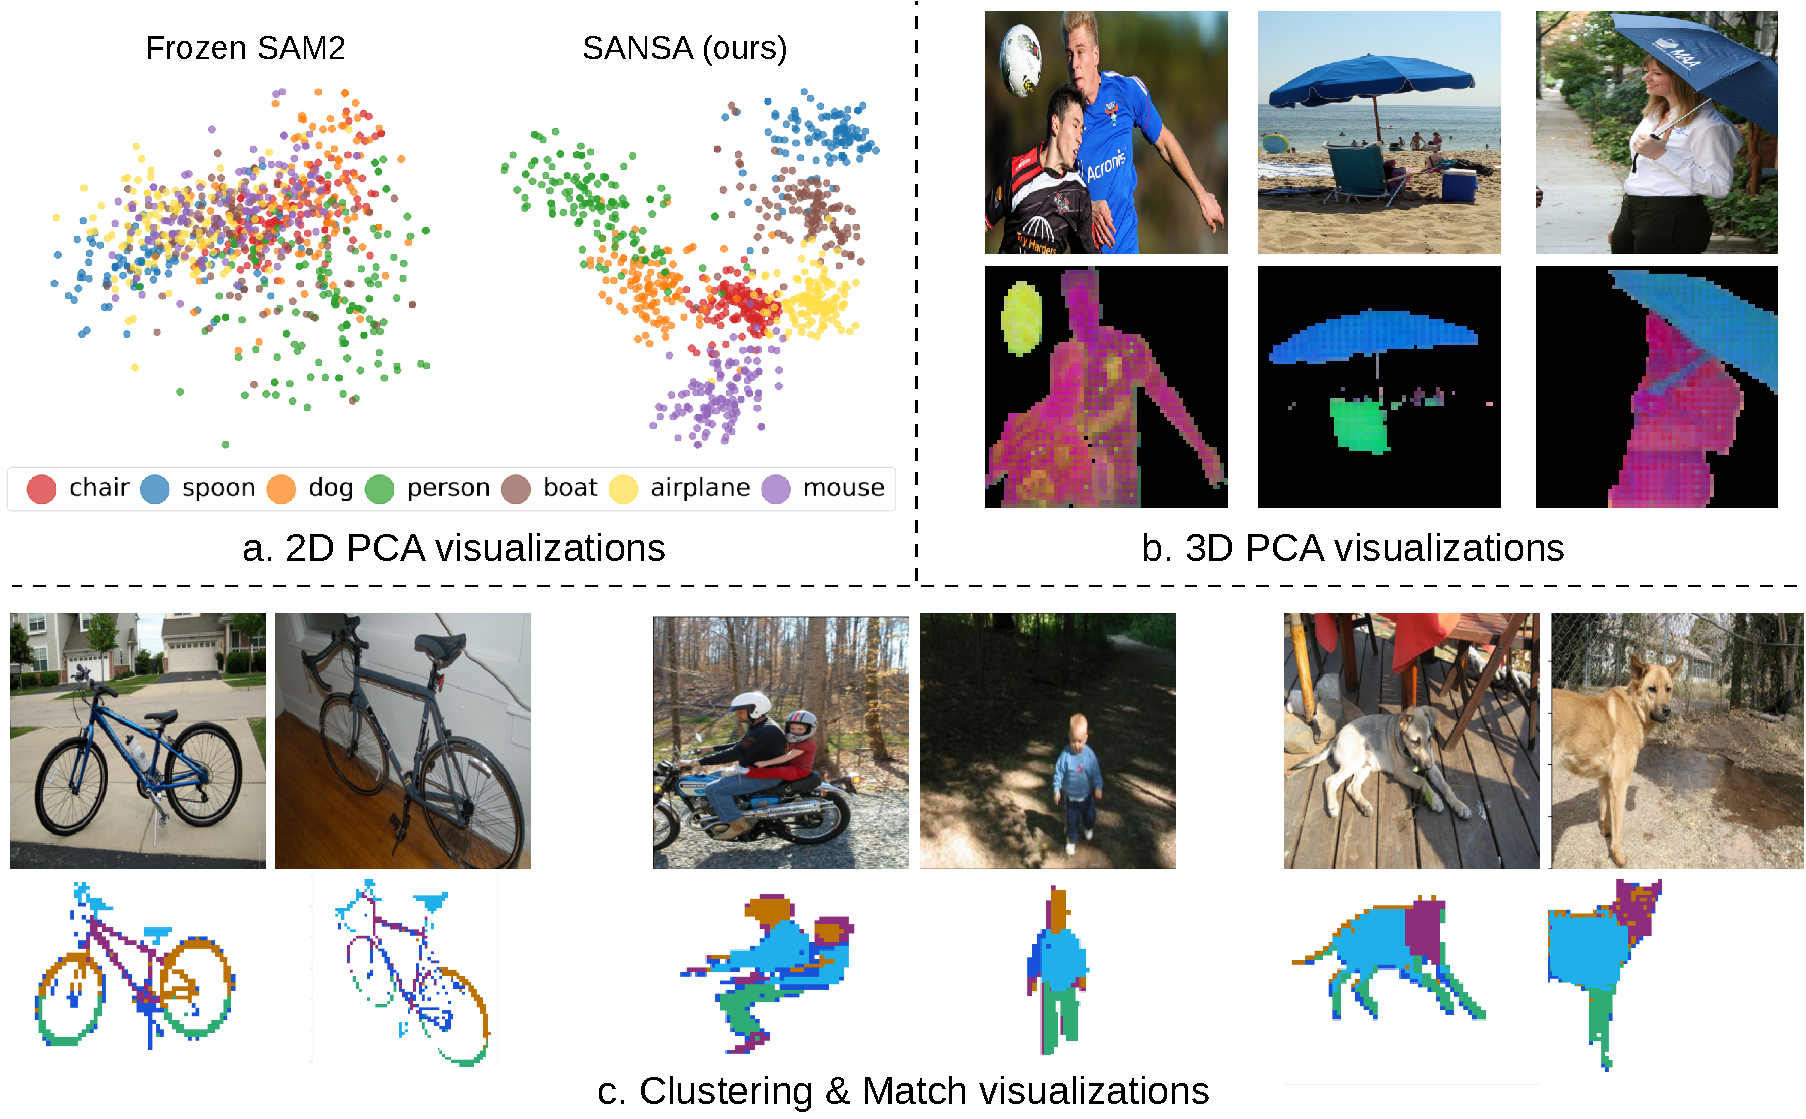
\includegraphics[width=0.9\linewidth]{images/semantic_correspondence.pdf}
    \caption{\textbf{Semantic structure of feature space.} (a) PCA visualization of frozen SAM2 and our \ours{} features on a COCO fold with \textit{unseen} classes, showing the first two principal components color-coded by class. SAM2 features exhibit weak semantic separability, indicating entanglement with other signals. (b) PCA-based RGB visualization of \ours{} features across images with \textit{seen} and \textit{unseen} categories, showing consistent semantic mapping. (c) Part-level semantics and cross-image consistency. We cluster features per object and match clusters across image pairs via Hungarian Matching. This reveals that \ours{} captures fine-grained distinctions (e.g., \textit{handlebar} vs. \textit{wheel}), spatial layout (e.g., \textit{upper} vs. \textit{lower wheel}), and produces representations that align across images.}
    \label{fig:semantic_correspondence}
    \vspace{-5pt}
\end{figure}
In \cref{fig:semantic_correspondence}b, we visualize \ours{} features using PCA, computed jointly across images, where the first three PCs are mapped to RGB channels. The visualization spans three images containing instances from both \textit{unseen} (e.g., person, chair, ball) and \textit{seen} (e.g., umbrella) categories. The consistent color mapping across instances of the same category highlights strong semantic grouping, mapping similar concepts coherently in feature space despite visual variability.

Finally, in \cref{fig:semantic_correspondence}c, we shift from coarse category level to fine-grained correspondences at the part level. 
Following \cite{zhang2023tale}, we cluster object features with \textit{K}-Means and match centroids across image pairs via the Hungarian Algorithm, then visualize matched clusters with shared colors to assess semantic consistency. The results show that, despite not being trained with part-level supervision, \ours{} features encode part-level understanding (\eg \textit{hand vs arm}, \textit{handlebar vs wheel}), spatial layout (\eg \textit{upper vs lower} wheel), and produce representations that align across images. \\

We provide an in-depth study of semantic representations in \cref{sec:supp_emergence}, using PCA, clustering, and linear probing to analyze how semantics are encoded in SAM2 and made explicit through adaptation.

